\subsection{Winery mit Docker}

Um Winery mit Docker zu deployen muss Docker zunächst installiert werden. Mittels Docker kann dann der Docker-Container von Winery deployed werden. Im Github Repository befindet sich ein Skript (\verb|deploy_docker.sh|) dafür. Der Einfachheit beim Aufruf halber haben wir den Port \verb|8080| des Containers an den Port \verb|80| der Hostmaschine gebunden. Winery kann also unter \verb|<HOST-IP>/winery)| aufgerufen werden.


\subsection{Moodle in Winery}
Abbildung \ref{fig:moodle_winery} zeigt die Topologie vom Moodle-CSAR, dargestellt von Winery.

\begin{figure}
\centering
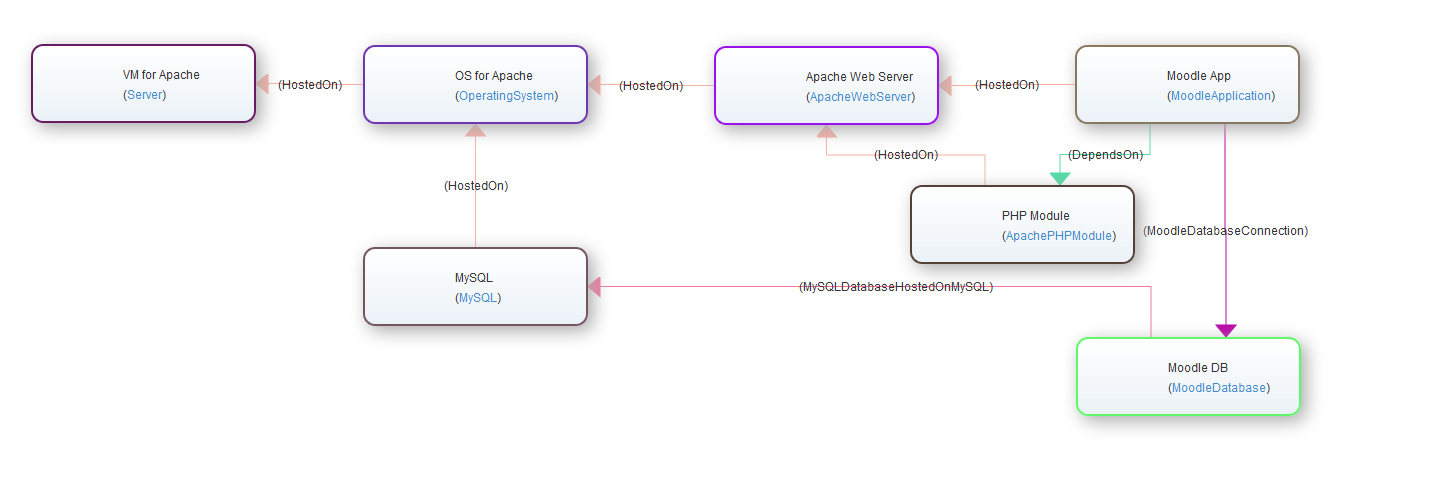
\includegraphics[width=\textwidth]{winery_moodle.png}
\caption{Moodle in Winery}
\label{fig:moodle_winery}
\end{figure}
\subsection{Moodle mittels OpenTOSCA}
Wie bereits auf der Mailing-Liste dargestellt, ist es derzeit nicht möglich, Moodle mittels OpenTOSCA zu instanziieren.
\subsubsection{Deployment von OpenTOSCA}
OpenTOSCA wurde von uns auf zwei verschiedenen Wegen deployed, zum einen mittels Amazon CloudFormation und zum anderen durch das in der Anleitung angegebene Shell-Skript (sowohl stable als auch unstable). Bei allen Varianten steht OpenTOSCA nach kurzer Zeit unter \verb|<SERVER-IP>:8080| zur Verfügung.
\subsubsection{Moodle mit OpenTOSCA}
Beim Deployment von Moodle treten laut Log (Error Logs im GitHub-Repository, \verb|sh-deploy_2015-05_error.log| (OpenTOSCA mittels Shell-Skript) und \verb|cf-deploy_2015-05_error.log| (OpenTOSCA mittels CloudFormation)) Fehler auf, obwohl im Webinterface angezeigt wird, dass das Deployment fehlerfrei war (siehe Abbildung \ref{fig:moodle_deployment}). Wenn Moodle jedoch im Folgenden mittels der Vinothek instantiiert werden soll, so schlägt dies fehl, das Webinterface bleibt bei "Instantiating Application... Please wait" hängen, im Log selbst tauchen keine Fehler oder weiterführende Informationen auf. Möglicherweise hängt dies nach der Bug-Beschreibung mit diesem Bug auf Github zusammen: \url{https://github.com/CloudCycle2/YAML_Transformer/issues/143}. Auch die vorgeschlagene Methode Moodle mittels SoapUI zu instantiieren schlägt fehl, da keine Verbindung aufgebaut werden kann. 

Eine weitere Beochbachtung ist, dass der Export von CSAR-Archiven aus der Winery fehlschlägt, zumindest sind diese erheblich kleiner als das zuvor importierte CSAR und OpenTOSCA bezeichnet das Archiv als beschädigt.
\begin{figure}
\centering
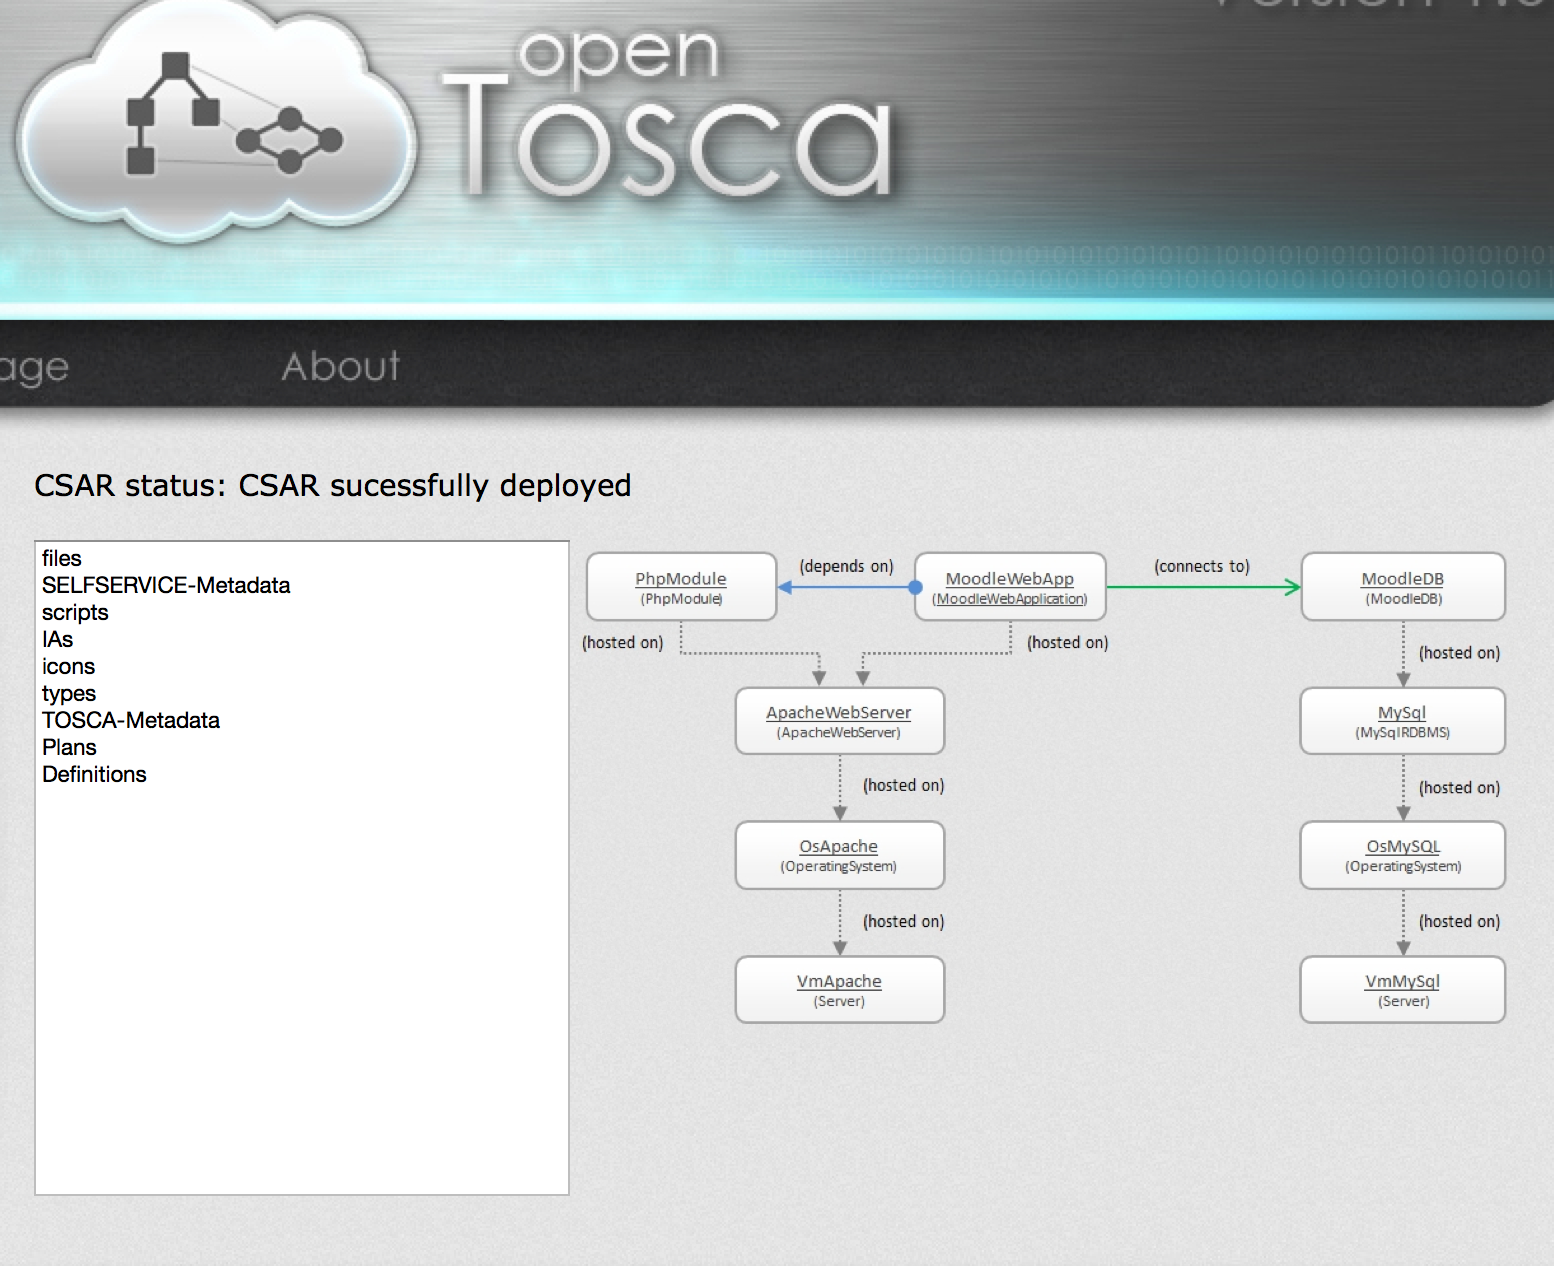
\includegraphics[width=\textwidth]{moodle_success.png}
\caption{Moodle Deployment}
\label{fig:moodle_deployment}
\end{figure}